\section{Neutrinos}

% - What are neutrinos?
Neutrinos are elementary particles with no electric charge and very little mass.
Their low interactivity
  makes them difficult to detect,
  but is also the reason why they are valuable messenger particles for cosmology:
Because they are not impacted by the electromagnetic force,
% and very little by gravity,
  their direction of travel is not affected by cosmic magnetic fields.
Neither does the interstellar medium absorb them in significant amounts.
Therefore,
  their direction of travel can be used to trace back the path of the matter that produced them.
Together with the energy of the neutrino,
  this information can be used to determine the properties of the matter that produced them.
This is the basis of neutrino astronomy.

% - What are their properties?

\subsection{Sources}
% - What are their sources?
%   - Nuclear reactors
%   - Solar
%   - AGNs
%   - Supernovae
%   - Atmospheric neutrinos
Neutrinos have various astronomical sources,
% \todo{We are not sure about these!}
including
  …. % TODO
  % supernovae,
  % pulsars, % Oxford comma
  % and active galactic nuclei.
Neutrinos are also produced in
  the Sun
  and in the Earth's atmosphere
  as well as in nuclear reactors.
They cover a wide range of energies, from a few \si{\mega\electronvolt} to a few \si{\tera\electronvolt},
  depending on the source.
%
\autoref{fig:neutrinos:flux_spectrum} shows the flux spectrum of neutrinos from different sources.
One can see
  the abundance of medium-energy neutrinos from the Sun,
    for example,
  as well as the scarcity of (hypothesized?) high-energy neutrinos from AGN,
    which \icecube is sensitive to.

\begin{figure}
  \centering
  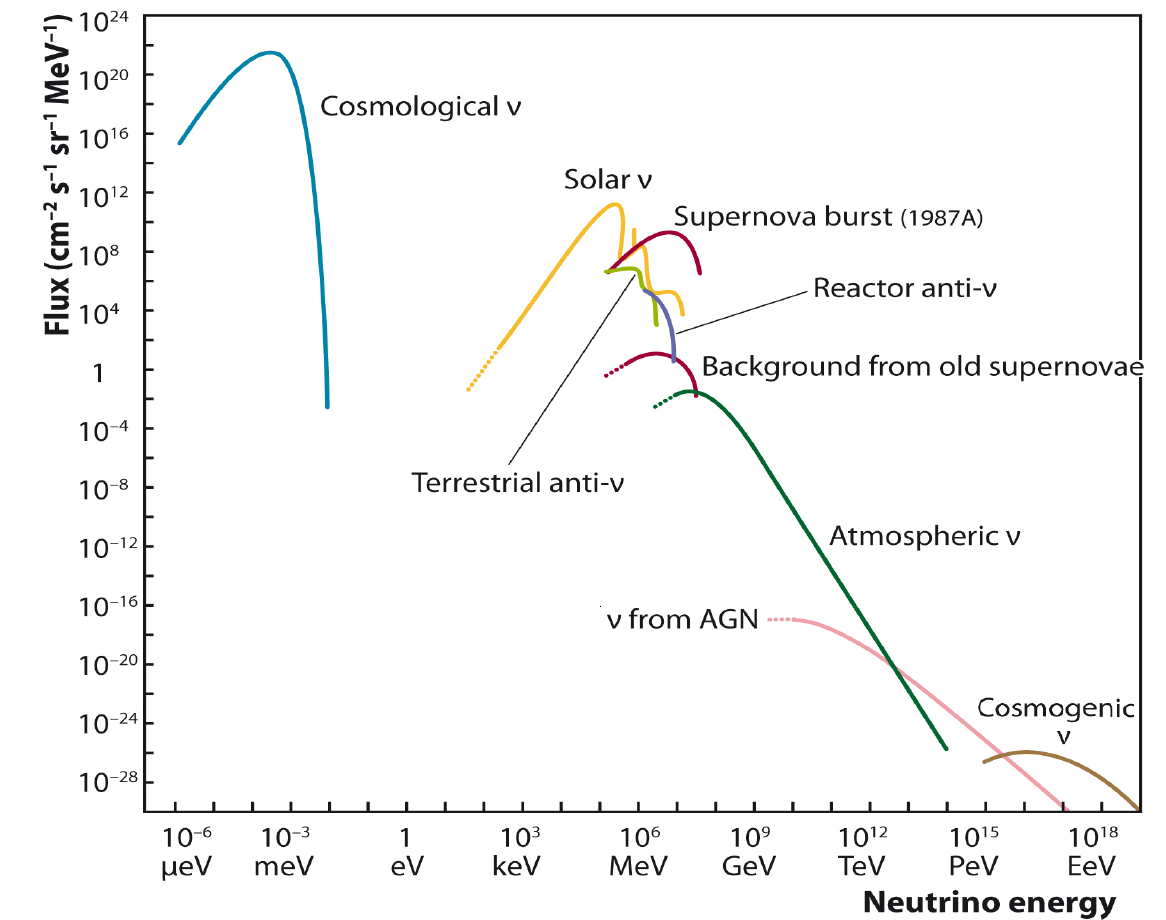
\includegraphics[width=0.75\textwidth]{content/plots/halftime/neutrinos-energy.png}
  \caption{Neutrino flux and corresponding source classes as a function of their energy. \citationneeded{}}
  \label{fig:neutrinos:flux_spectrum}
\end{figure}


\subsection{Neutrino oscillations}
While current models of neutrino sources predict a ratio of
  $\nu_e:\nu_\mu:\nu_\tau = 1:2:0$,
the observed ratio on Earth is
  $\nu_e:\nu_\mu:\nu_\tau = 1:1:1$.
This discrepancy is explained by neutrino oscillations \cite{neutrinos_beacom},
  which are a consequence of the fact that neutrinos have mass.
The mass of the neutrinos is very small,
  but it is large enough to cause oscillations between the different flavors,
  given the large distances that cosmic neutrinos travel.


% - What are their interactions?
%   - Weak interaction
\subsection{Interaction with matter}
  \todo{Move to IceCube?}
Neutrinos interact with matter via the weak interaction.
In order to compensate for the low cross-section of the weak interaction,
  the effective detector volume is maximized by utilizing existing naturally occurring detector materials,
  such as
    the Earth's atmosphere,
    the sea,
    or the ice in the Antarctic.

% - How are they detected?
%   - → IceCube, later
